%!TEX program = xelatex
%Template created by: Maciej Byczko
\documentclass[a4paper,12pt]{extarticle}  %typ dokumentu

% \usepackage[utf8]{inputenc} %rodzaj czcionki w dokumencie
\usepackage{geometry} %poprawienie marginesów
\usepackage{polski} %polskie znaki
\usepackage{multirow} %tabela
\usepackage{graphicx} %tabela
\usepackage{float} %poprawienie pozycji
\usepackage{fancyhdr} % header i footer
\usepackage{karnaugh-map} % rysowanie siatek karnaugh
\usepackage{hyperref} %tworzenie odnośników, \url{<url>}, \href{<file path, link>}{<text with link>} \pageref{}
\usepackage{amsmath} % Matma
\usepackage{boldline}%edytowanie grubości krawędzi w tabelach \hlineB{} \clineB{}{}
\usepackage{array}%grubsze kolumny w tabeli
\usepackage{bigstrut}
\usepackage{caption}
\usepackage{listings} %pisanie kodu w ładny sposób, begin{listings}[language=<język>]...end{listings} tak samo jak nazwa paczki
\usepackage{subcaption}

%Ustawienie paczki hyperref
\hypersetup{
     colorlinks,
     citecolor=black,
     filecolor=black,
     linkcolor=black,
     urlcolor=black
}

\definecolor{backcolour}{rgb}{0.95,0.95,0.92}
\definecolor{AO}{rgb}{0,0.5,0}
\definecolor{ZeroBlue}{rgb}{0,0.28,0.73}
\definecolor{DarkRed}{rgb}{0.85,0.16,0.16}

\lstset{
breaklines=true,
language=vhdl,
numbers=left,
tabsize=2,
numberstyle=\tiny,
backgroundcolor=\color{backcolour},
breakatwhitespace=false,
showspaces=false,                
showstringspaces=false,
showtabs=false,
commentstyle=\color{gray},
keywordstyle=\color{ZeroBlue},
% keywordstyle={[2]\color{DarkRed}},
% keywordstyle={[3]\color{ZeroBlue}},
}
\graphicspath{{pictures/}}
\geometry{margin=0.7in}
\pagestyle{fancy}

\cfoot{Strona \thepage}
\rhead{Strona \thepage}
\lhead{\typdoc}
\newcolumntype{?}{!{\vrule width 1.5pt}}

\title{\tytul}
\author{\tworcy}
\date{\data}

%-----------------------PRZYDATNE LINKI----------------------------------
%link do tworzenia tabeli https://tablesgenerator.com
%symbole matematyczne: https://oeis.org/wiki/List_of_LaTeX_mathematical_symbols
%narzędzia matematyczne: https://en.wikibooks.org/wiki/LaTeX/Mathematics
%krótkie podpowiedzi http://www.mif.pg.gda.pl/homepages/sylas/students/wdi/doc/latex-sciaga.html
%symbole do schematów: http://texdoc.net/texmf-dist/doc/latex/circuitikz/circuitikzmanual.pdf
%----------------------------------------------------------------------

%-----------------------SEKCJA DANYCH----------------------------------
\def\tytul{Układy wielobitowych wejść i wyjść} %<<< tytuł ćwiczenia
\def\nrcw{4} %<<< numer ćwiczenia
\def\data{8 Listopada 2021r.} %<< data wykonania
\def\prowadzacy{dr inż. Jacek Mazurkiewicz} %<<<prowadzący
\def\nrgrupy{B} %<<<numer grupy
\def\tworcy{Maciej Byczko\\Bartosz Matysiak} %<<< autorzy
\def\zajinfo{PN 10:50 TP} %<<< informacje dotyczące zajęć
\def\typdoc{Sprawozdanie} %<<< typ dokumentu tj Sprawozdanie, zadania itp. {Matematyka dyskretna/Sprawozdanie z Miernictwa}
\begin{document}
\setlength{\headheight}{15pt}

\newcommand{\ov}[1]{\overline{#1} \ }

%-------------------------------------TABELA-DANYCH--------------------------------------------------
\begin{table}[H]
	\centering
	\resizebox{\textwidth}{!}{
		\begin{tabular}{|c|c|c|}\hline
			\begin{tabular}[c]{@{}c@{}}                     \tworcy     \end{tabular} &
			\begin{tabular}[c]{@{}c@{}}Prowadzący:\\        \prowadzacy \end{tabular} &
			\begin{tabular}[c]{@{}c@{}}Numer ćwiczenia\\    \nrcw       \end{tabular}          \\ \hline
			\begin{tabular}[c]{@{}c@{}}                     \zajinfo    \end{tabular} &
			\begin{tabular}[c]{@{}c@{}}Temat ćwiczenia:\\   \tytul      \end{tabular} & Ocena: \\ \hline
			\begin{tabular}[c]{@{}c@{}}Grupa:\\          \nrgrupy    \end{tabular}    &
			\begin{tabular}[c]{@{}c@{}}Data wykonania:\\    \data       \end{tabular} &        \\ \hline
		\end{tabular}}
\end{table}
%----------------------------------------------------------------------------------------------------
\tableofcontents
\cleardoublepage
\section{Zadanie 1}
\subsection{Polecenie}
Detektor 2-znakowej sekwencji słów 8-bitowych: wejścia 2 znaków 8-bitowych, 
1 wyjście 1-bitowe – sekwencja rozpoznana / sekwencja błędna. Źródło danych: 
początkowo "guziki" przystawki, potem klawiatura PC via terminal. 
\subsection{Rozwiązanie}
Do rozwiązania problemu wymagane jest od nas podłączenie dwóch komparatorów 8-bitowych (COMP8), 
które po pobraniu wartości od użytkownika kolejno po sobie sprawdzają wprowadzone słowa.

Aby wymusić na użytkowniku wprowadzanie odpowiedniej kolejności wpisywania wartości zastosowaliśmy przerzutnik typu "D" aby wytworzyć opóźnienie.

\subsubsection{Schemat układu}
Schemat dla wersji z przyciskami jako wejściem:
\begin{figure}[H]
	\centering
	\resizebox*{\textwidth}{!}{
		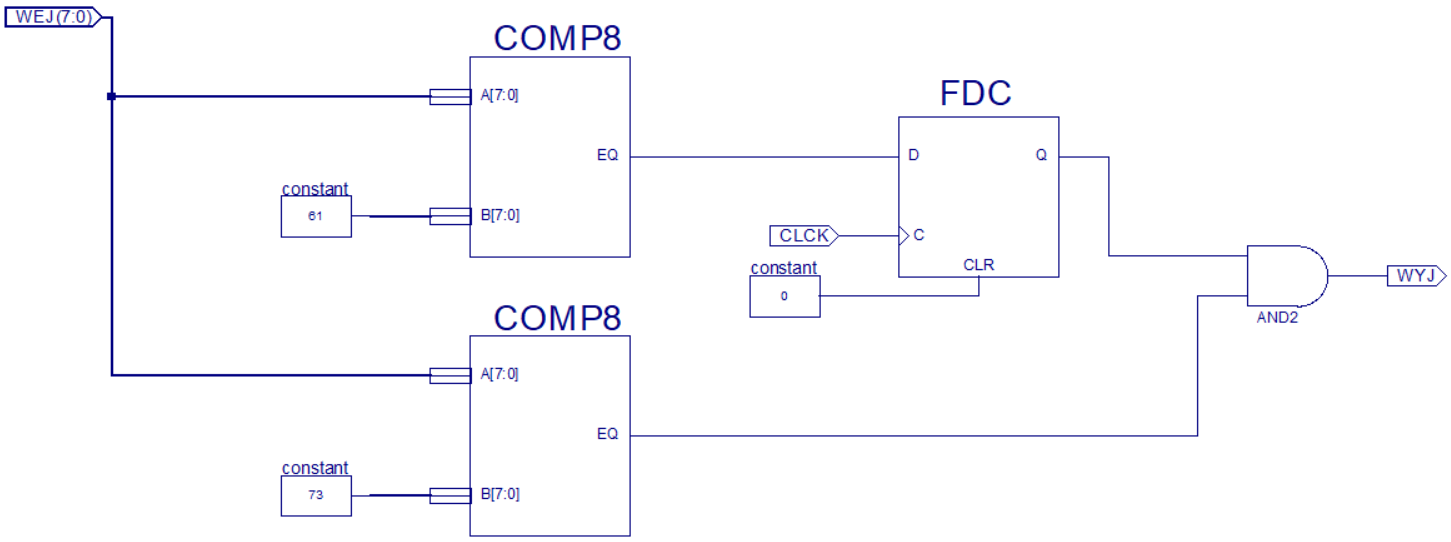
\includegraphics{zadanie1/zad1_scheme_button_input.png}
	}
\end{figure}
\subsubsection{Kod VHDL}
\lstinputlisting{zadanie1/testbench.vhd}
\subsubsection{Symulacja}
\begin{figure}[H]
	\centering
	\resizebox*{\textwidth}{!}{
		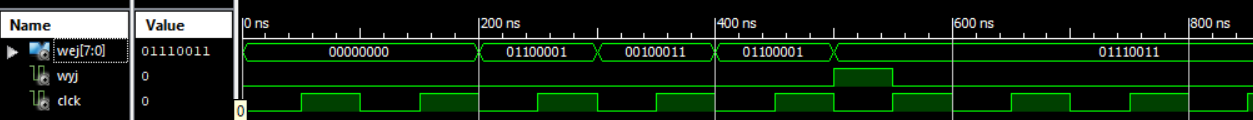
\includegraphics{zadanie1/zad1_simulation.png}
	}
\end{figure}
\subsection{Fizyczna implementacja}
\subsubsection{Kod UCF}
\lstinputlisting{zadanie1/zad1_button_input.ucf}
\subsection{Implementacja klawiatury}
Aby wykorzystać klawiaturę komputera jako źródło danych via terminal, musieliśmy zaimportować moduł RS232\_RX ze strony laboratorium.

Aby moduł został poprawnie zaimplementowany musieliśmy go umieścić na schemacie, 
wczytać nowe wejścia do pliku VHDL oraz przypisać te wejścia do 
odpowiednich elementów zestawu fizycznego za pomocą pliku UCF.
\subsubsection{Schemat układu}
\begin{figure}[H]
	\centering
	\resizebox*{\textwidth}{!}{
		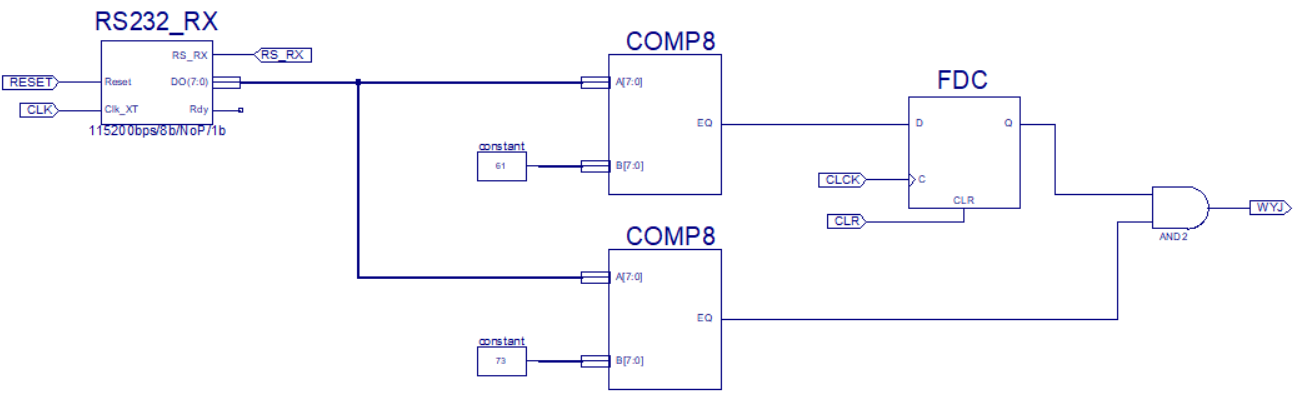
\includegraphics{zadanie1/zad1_scheme_keyboard_input.png}
	}
\end{figure}
\subsubsection{Kod VHDL}
\lstinputlisting{zadanie1/testbench_keyboard.vhd}
\subsubsection{Kod UCF}
\lstinputlisting{zadanie1/zad1_keyboard_input.ucf}

Zadanie zostało wykonane bez większych komplikacji, z powodu sposobu implementacji poprawną kombinację (a,s) musimy wpisać odpowiednio szybko oraz w tym samym tempie co zegar podłączony do przerzutnika.
\section{Zadanie 2}
\subsection{Polecenie}
Układ arytmetyczny pracujący na dwóch argumentach 4-bitowych wyrażonych w kodzie Aikena
i generujący stosowny wynik w tymże kodzie. 
\subsection{Rozwiązanie}
Najłatwiejszym sposobem na wykonanie dodawania dwóch liczb w kodzie Aikena okazała się zamiana danych wejściowych na NKB.
Cyfry 0-4 pokrywają się w obu kodach, więc musieliśmy zamienić jedynie cyfry 5-9.
Zauważyliśmy że aby sprawnie wykonać tą zmianę, musieliśmy odjąć wartość 0110 (6) aby uzyskać wymaganą wartość binarną.
Operandy już skonwertowane na NKB dodajemy przy pomocy zwykłego sumatora. Otrzymany wynik ponownie konwertujemy na kod Aikena, wykrywając także, czy należy on do dziedziny tego kodu, i sygnalizując to wyjściem przepełnienia.
Potrzebne są zatem dwa typy podukładów: konwerter kodu Aikena na NKB, i konwerter odwrotny, z dodatkowym wyjściem przepełnienia. 

Ustaliliśmy, że w momencie przepełnienia, czyli gdy wartość 9 zostanie przekroczona, zapala się lampka przepełnienia informująca, że wynik jest niewiarygodny (nieważny).

%\subsubsection{Schemat stanów} % pozwolę sobie zauważyć, że stanów, w układach kombinacyjnych, takim jak ten, nie ma
%Dałbym bardziej cos w rodzaju notki wstępnej, np.
% \subsection{Uwagi wstępne}
% i tu opis ogólnej struktury układu

\subsubsection{Tabele prawdy} %liczba mnoga; tabele dla każdego podukładu

\begin{table}[H]
	\centering
	\caption{Konwerter kod Aikena - > NKB}
	\resizebox*{0.8\textwidth}{!}{
		\begin{tabular}{|c|c|c|c?c|c|c|c|}
		\hline
		$A_3$ & $A_2$ & $A_1$ & $A_0$ & $Y_3$ & $Y_2$ & $Y_1$ & $Y_0$ \\ \hlineB{2.5}
		0    & 0    & 0    & 0    & 0    & 0    & 0    & 0    \\ \hline
		0    & 0    & 0    & 1    & 0    & 0    & 0    & 1    \\ \hline
		0    & 0    & 1    & 0    & 0    & 0    & 1    & 0    \\ \hline
		0    & 0    & 1    & 1    & 0    & 0    & 1    & 1    \\ \hline
		0    & 1    & 0    & 0    & 0    & 1    & 0    & 0    \\ \hline
		0    & 1    & 0    & 1    & -    & -    & -    & -    \\ \hline
		0    & 1    & 1    & 0    & -    & -    & -    & -    \\ \hline
		0    & 1    & 1    & 1    & -    & -    & -    & -    \\ \hline
		1    & 0    & 0    & 0    & -    & -    & -    & -    \\ \hline
		1    & 0    & 0    & 1    & -    & -    & -    & -    \\ \hline
		1    & 0    & 1    & 0    & -    & -    & -    & -    \\ \hline
		1    & 0    & 1    & 1    & 0    & 1    & 0    & 1    \\ \hline
		1    & 1    & 0    & 0    & 0    & 1    & 1    & 0    \\ \hline
		1    & 1    & 0    & 1    & 0    & 1    & 1    & 1    \\ \hline
		1    & 1    & 1    & 0    & 1    & 0    & 0    & 0    \\ \hline
		1    & 1    & 1    & 1    & 1    & 0    & 0    & 1    \\ \hline
		\end{tabular}
	}
\end{table}

\begin{table}[H]
	\centering
	\caption{Konwerter NKB - > kod Aikena}
	\resizebox*{0.8\textwidth}{!}{
		\begin{tabular}{|c|c|c|c|c?c?c|c|c|c|}
		\hline
		$S_4$ & $S_3$ & $S_2$ & $S_1$ & $S_0$ & $OVL$ & $Y_3$ & $Y_2$ & $Y_1$ & $Y_0$ \\ \hlineB{2.5}
		0     & 0     & 0     & 0     & 0     & 0     & 0     & 0     & 0     & 0 \\ \hline
		0     & 0     & 0     & 0     & 1     & 0     & 0     & 0     & 0     & 1 \\ \hline
		0     & 0     & 0     & 1     & 0     & 0     & 0     & 0     & 1     & 0 \\ \hline
		0     & 0     & 0     & 1     & 1     & 0     & 0     & 0     & 1     & 1 \\ \hline
		0     & 0     & 1     & 0     & 0     & 0     & 0     & 1     & 0     & 0 \\ \hline
		0     & 0     & 1     & 0     & 1     & 0     & 1     & 0     & 1     & 1 \\ \hline
		0     & 0     & 1     & 1     & 0     & 0     & 1     & 1     & 0     & 0 \\ \hline
		0     & 0     & 1     & 1     & 1     & 0     & 1     & 1     & 0     & 1 \\ \hline
		0     & 1     & 0     & 0     & 0     & 0     & 1     & 1     & 1     & 0 \\ \hline
		0     & 1     & 0     & 0     & 1     & 0     & 1     & 1     & 1     & 1 \\ \hline
		0     & 1     & 0     & 1     & 0     & 1     & -     & -     & -     & - \\ \hline
		0     & 1     & 0     & 1     & 1     & 1     & -     & -     & -     & - \\ \hline
		0     & 1     & 1     & 0     & 0     & 1     & -     & -     & -     & - \\ \hline
		0     & 1     & 1     & 0     & 1     & 1     & -     & -     & -     & - \\ \hline
		0     & 1     & 1     & 1     & 0     & 1     & -     & -     & -     & - \\ \hline
		0     & 1     & 1     & 1     & 1     & 1     & -     & -     & -     & - \\ \hline
		1     & 0     & 0     & 0     & 0     & 1     & -     & -     & -     & - \\ \hline
		1     & 0     & 0     & 0     & 1     & 1     & -     & -     & -     & - \\ \hline
		1     & 0     & 0     & 1     & 0     & 1     & -     & -     & -     & - \\ \hline
		\end{tabular}%
	}
	%\label{tab:addlabel}%
  \end{table}%

  Wejściem układu są bity S(4:0), stanowiące wyjście sumatora czterobitowego (S(3:0) - bity cyfr wyjściowych sumatora, $S_{4}$ - bit Carry Out tegoż). Można zauważyć, że bit przepełnienia jest jedynką wtedy i tylko wtedy, gdy ustawiony jest bit $S_4$ lub gdy bity S(3:0) tworzą liczbę większą od 9 (w NKB); dzięki temu spostrzeżeniu (bezpośrednio potem oddanego na schemacie), możliwe stało się zredukowanie liczby argumentów funkcji logicznej z pięciu do czterech. Pozostałe bity wyjściowe również są funkcjami czterech bitów S(3:0), co umożliwia skonstruowanie przejrzystych siatek Karnaugh.

%\begin{table}[H]
%    \centering
%    \caption{Konwerter kod Aikena -> NKB}
%    \resizebox*{\textwidth}{!}{
%      \begin{tabular}{|c?c|c|c?c?c|c|c?c?c|c|c|}
%      \hline
%      \multirow{2}[4]{*}{S} & \multicolumn{3}{c?}{Q(t)} & \multirow{2}[4]{*}{Z} & \multicolumn{3}{c?}{Q(t+1)} & \multirow{2}[4]{*}{Y} & \multicolumn{3}{c|}{T(t)} \bigstrut\\
%  	  \clineB{2-4}{2.5}\clineB{6-8}{2.5}\clineB{10-12}{2.5}      & $Q_2$ & $Q_1$ & $Q_0$ &   & $Q_2$ & $Q_1$ & $Q_0$ &   & $T_2$ & $T_1$ & $T_0$ \bigstrut\\
%	  \hlineB{2.5}
%      $Q_0$ & 0 & 0 & 0 & 0 & 0 & 0 & 0 & 0 & 0 & 0 & 0 \bigstrut\\
%      \hline
%      $Q_0$ & 0 & 0 & 0 & 1 & 0 & 0 & 1 & 0 & 0 & 0 & 1 \bigstrut\\
%      \hline
%      $Q_1$ & 0 & 0 & 1 & 0 & 0 & 0 & 0 & 0 & 0 & 0 & 1 \bigstrut\\
%      \hline
%      $Q_1$ & 0 & 0 & 1 & 1 & 0 & 1 & 0 & 0 & 0 & 1 & 1 \bigstrut\\
%      \hline
%      $Q_2$ & 0 & 1 & 0 & 0 & 0 & 1 & 1 & 0 & 0 & 0 & 1 \bigstrut\\
%      \hline
%      $Q_2$ & 0 & 1 & 0 & 1 & 0 & 1 & 0 & 0 & 0 & 0 & 0 \bigstrut\\
%      \hline
%      $Q_3$ & 0 & 1 & 1 & 0 & 0 & 0 & 0 & 0 & 0 & 1 & 1 \bigstrut\\
%      \hline
%      $Q_3$ & 0 & 1 & 1 & 1 & 1 & 0 & 0 & 0 & 1 & 1 & 1 \bigstrut\\
%      \hline
%      $Q_4$ & 1 & 0 & 0 & 0 & 0 & 0 & 0 & 0 & 1 & 0 & 0 \bigstrut\\
%      \hline
%      $Q_4$ & 1 & 0 & 0 & 1 & 1 & 0 & 1 & 0 & 0 & 0 & 1 \bigstrut\\
%      \hline
%      $Q_5$ & 1 & 0 & 1 & 0 & 0 & 1 & 1 & 1 & 1 & 1 & 0 \bigstrut\\
%      \hline
%      $Q_5$ & 1 & 0 & 1 & 1 & 0 & 1 & 0 & 1 & 1 & 1 & 1 \bigstrut\\
%      \hline
%      - & 1 & 1 & 0 & 0 & - & - & - & - & - & - & - \bigstrut\\
%      \hline
%      - & 1 & 1 & 0 & 1 & - & - & - & - & - & - & - \bigstrut\\
%      \hline
%      - & 1 & 1 & 1 & 0 & - & - & - & - & - & - & - \bigstrut\\
%      \hline
%      - & 1 & 1 & 1 & 1 & - & - & - & - & - & - & - \bigstrut\\
%      \hline
%      \end{tabular}%
%    }
%    \label{tab:mealy}%
%  \end{table}

\newpage

\subsubsection{Siatki Karnaugh}
	Konwerter kod Aikena - > NKB:
	\begin{figure}[H]
    \centering
    \begin{minipage}[c]{0.49\linewidth}
    \begin{karnaugh-map}[4][4][1][$A_1A_0$][$A_3A_2$]
    \minterms{14,15}
    \maxterms{0,1,2,3,4,11,12,13}
    \autoterms[-] % umieść ten symbol w miejscach niezdefiniowanych
    \implicant{7}{14}
    %\implicantedge{12}{8}{14}{10}
    %\implicant{15}{10}
    % \minterms{0} % na tych koordynatach umieść jedynki (1)
    % \maxterms{1,2,3,4}
    % \implicantedge{0}{0}{8}{8}
    \end{karnaugh-map}
    \centering
    \vspace{-1cm}
    \hspace{1cm}
    \caption*{$Y_3 = A_2A_1$}
    \end{minipage}
    \centering
    \begin{minipage}[c]{0.49\linewidth}
	\begin{karnaugh-map}[4][4][1][$A_1A_0$][$A_3A_2$]
    \minterms{4,11,12,13}
    \maxterms{0,1,2,3,14,15}
    \autoterms[-] % umieść ten symbol w miejscach niezdefiniowanych
    \implicant{4}{13}
    \implicant{8}{10}
    %\implicant{15}{10}
    % \minterms{0,11} % na tych koordynatach umieść jedynki (1)
    % \maxterms{1,2,3}
    % \implicant{0}{8}
    % \implicant{12}{10}
    \end{karnaugh-map}
    \centering
    \vspace{-1cm}
    \hspace{1cm}
    \caption*{$Y_2 = A_3\ov{A_2} + A_2\ov{A_1}$}
    \end{minipage}
    \end{figure}
	\vspace{-1cm}
	\begin{figure}[H]
		\centering
		\begin{minipage}[c]{0.49\linewidth}
		\begin{karnaugh-map}[4][4][1][$A_1A_0$][$A_3A_2$]
		\minterms{2,3,12,13}
		\maxterms{0,1,4,11,14,15}
		\autoterms[-] % umieść ten symbol w miejscach niezdefiniowanych
		\implicant{3}{6}
		%\implicantedge{12}{8}{14}{10}
		\implicant{12}{9}
		% \minterms{0} % na tych koordynatach umieść jedynki (1)
		% \maxterms{1,2,3,4}
		% \implicantedge{0}{0}{8}{8}
		\end{karnaugh-map}
		\centering
		\vspace{-1cm}
		\hspace{1cm}
		\caption*{$Y_1 = A_3\ov{A_1} + \ov{A_3}A_1= A_3 \oplus A_1$}
		\end{minipage}
		\centering
		\begin{minipage}[c]{0.49\linewidth}
		\begin{karnaugh-map}[4][4][1][$A_1A_0$][$A_3A_2$]
		\minterms{1,3,11,13,15}
		\maxterms{0,2,4,12,14}
		\autoterms[-] % umieść ten symbol w miejscach niezdefiniowanych
		\implicant{1}{11}
		%\implicant{7}{14}
		%\implicant{15}{10}
		% \minterms{0,11} % na tych koordynatach umieść jedynki (1)
		% \maxterms{1,2,3}
		% \implicant{0}{8}
		% \implicant{12}{10}
		\end{karnaugh-map}
		\centering
		\vspace{-1cm}
		\hspace{1cm}
		\caption*{$Y_0 = A_0$}
		\end{minipage}
		\end{figure}

		\begin{center}
			Konwerter NKB - > kod Aikena:
		\end{center}

		\begin{figure}[H]
			\centering
			\begin{minipage}[c]{0.49\linewidth}
			\begin{karnaugh-map}[4][4][1][$S_1S_0$][$S_3S_2$]
			\minterms{10,11,12,13,14,15}
			\maxterms{0,1,2,3,4,5,6,7,8,9}
			\autoterms[-] % umieść ten symbol w miejscach niezdefiniowanych
			\implicant{12}{14}
			%\implicantedge{12}{8}{14}{10}
			\implicant{15}{10}
			% \minterms{0} % na tych koordynatach umieść jedynki (1)
			% \maxterms{1,2,3,4}
			% \implicantedge{0}{0}{8}{8}
			\end{karnaugh-map}
			\centering
			\vspace{-1cm}
			\hspace{1cm}
			\caption*{$OVL = S_3S_2 + S_3S_1 =S_3(S_2+S_1)$}
			\end{minipage}
		\end{figure}

		\vspace{-1cm}

		\begin{figure}[H]
			\centering
			\begin{minipage}[c]{0.49\linewidth}
			\begin{karnaugh-map}[4][4][1][$S_1S_0$][$S_3S_2$]
			\minterms{5,6,7,8,9}
			\maxterms{0,1,2,3,4}
			\autoterms[-] % umieść ten symbol w miejscach niezdefiniowanych
			\implicant{12}{10}
			\implicant{5}{15}
			\implicant{7}{14}
			
			%\implicantedge{12}{8}{14}{10}
			%\implicant{15}{10}
			% \minterms{0} % na tych koordynatach umieść jedynki (1)
			% \maxterms{1,2,3,4}
			% \implicantedge{0}{0}{8}{8}
			\end{karnaugh-map}
			\centering
			\vspace{-1cm}
			\hspace{1cm}
			\caption*{$R_3 = S_3+S_2S_1+S_2S_0$}
			\end{minipage}
			\centering
			\begin{minipage}[c]{0.49\linewidth}
			\begin{karnaugh-map}[4][4][1][$S_1S_0$][$S_3S_2$]
			\minterms{4,6,7,8,9}
			\maxterms{0,1,2,3,5}
			\autoterms[-] % umieść ten symbol w miejscach niezdefiniowanych
			\implicant{12}{10}
			\implicant{7}{14}
			\implicantedge{4}{12}{6}{14}
			%\implicant{8}{10}
			%\implicant{15}{10}
			% \minterms{0,11} % na tych koordynatach umieść jedynki (1)
			% \maxterms{1,2,3}
			% \implicant{0}{8}
			% \implicant{12}{10}
			\end{karnaugh-map}
			\centering
			\vspace{-1cm}
			\hspace{1cm}
			\caption*{$R_2 = S_3+S_2S_1+S_2\ov{S_0}$}
			\end{minipage}
			\end{figure}

			\vspace{-1cm}

			\begin{figure}[H]
				\centering
				\begin{minipage}[c]{0.49\linewidth}
				\begin{karnaugh-map}[4][4][1][$S_1S_0$][$S_3S_2$]
				\minterms{2,3,5,8,9}
				\maxterms{0,1,4,6,7}
				\autoterms[-] % umieść ten symbol w miejscach niezdefiniowanych
				%\implicant{3}{6}
				%\implicantedge{12}{8}{14}{10}
				\implicantedge{3}{2}{11}{10}
				\implicant{12}{10}
				\implicant{5}{13}
				% \minterms{0} % na tych koordynatach umieść jedynki (1)
				% \maxterms{1,2,3,4}
				% \implicantedge{0}{0}{8}{8}
				\end{karnaugh-map}
				\centering
				\vspace{-1cm}
				\hspace{1cm}
				\caption*{$R_1 = S_3+\ov{S_2}S_1+S_2\ov{S_1}S_0$}
				\end{minipage}
				\centering
				\begin{minipage}[c]{0.49\linewidth}
				\begin{karnaugh-map}[4][4][1][$S_1S_0$][$S_3S_2$]
				\minterms{1,3,5,7,9}
				\maxterms{0,2,4,6,8}
				\autoterms[-] % umieść ten symbol w miejscach niezdefiniowanych
				\implicant{1}{11}
				%\implicant{7}{14}
				%\implicant{15}{10}
				% \minterms{0,11} % na tych koordynatach umieść jedynki (1)
				% \maxterms{1,2,3}
				% \implicant{0}{8}
				% \implicant{12}{10}
				\end{karnaugh-map}
				\centering
				\vspace{-1cm}
				\hspace{1cm}
				\caption*{$R_0 = S_0$}
				\end{minipage}
				\end{figure}

				


\subsubsection{Schemat układu}
\begin{figure}[H]
	\centering
	\resizebox*{\textwidth}{!}{
		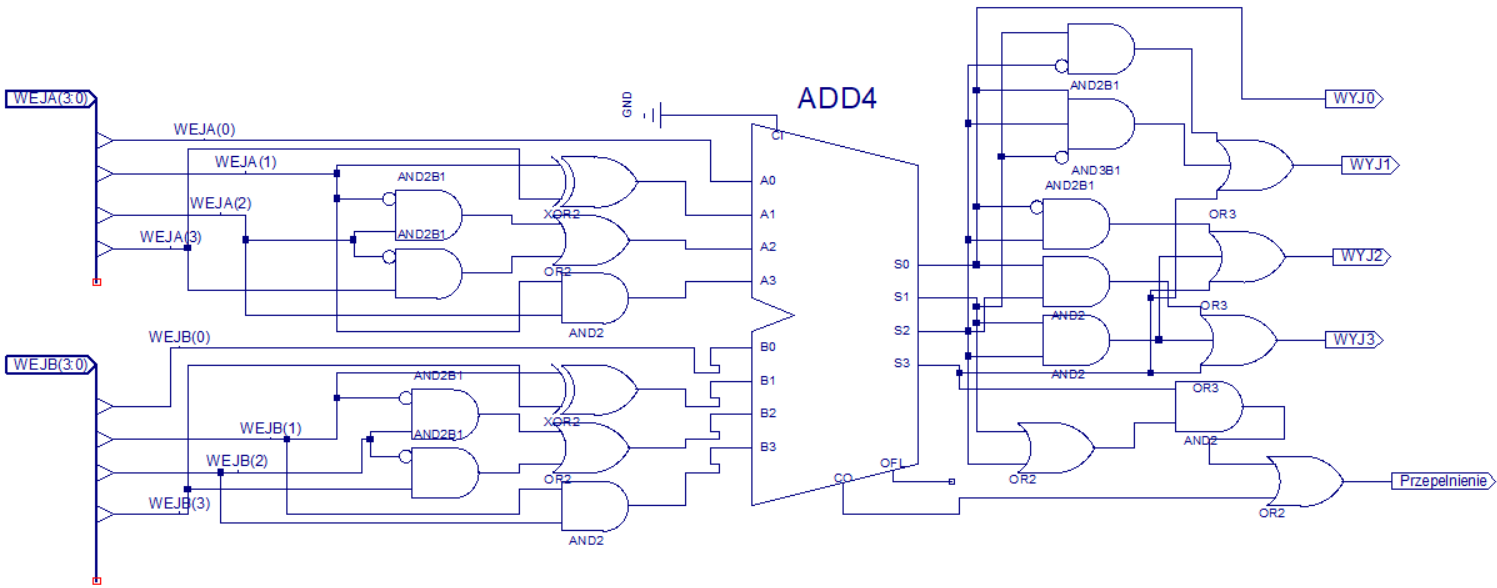
\includegraphics{zadanie2/zad2_scheme.png}
	}
\end{figure}
\subsubsection{Kod VHDL}
\lstinputlisting{zadanie2/testbench.vhd}
\subsubsection{Symulacja}
\begin{figure}[H]
	\centering
	\resizebox*{\textwidth}{!}{
		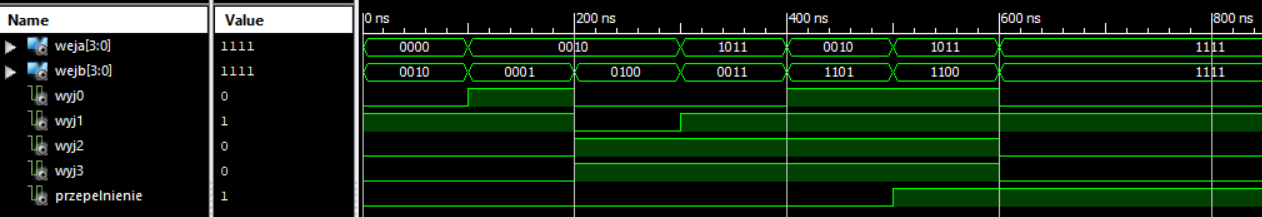
\includegraphics{zadanie2/zad2_simulation.png}
	}
\end{figure}
\subsection{Fizyczna implementacja}
\subsubsection{Kod UCF}
\lstinputlisting{zadanie2/ZL-9572.ucf}

W tej implementacji dodawanie następowało w czasie rzeczywistym, panel przycisków został podzielony na 2 sekcje dzięki czemu mogliśmy bezproblemowo wprowadzać 4-bitowe wartości.
\section{Zadanie 3}
\subsection{Polecenie}
Konwerter cyfry szesnastkowej zapisanej na czterech bitach od 0 do 9, A do F 
na kod ASCII tej cyfry – wyjście 8-bitowe. Prezentacja wyniku na diodach 
przystawki, potem na wyświetlaczu 7-segmentowym. 
\subsection{Rozwiązanie}
W celu dokonania konwersji, układ sprawdza czy prowadzona cyfra posiada wartość mniejszą niż 10. W celu uzyskania kodu ASCII w takim wypadku należy dodać 48 do wprowadzonej wartości.
W przeciwnym razie należy dodać 55.
Schemat działa na podobnej zasadzie co sumator z zadania 2 - wynik konwersji jest podawany na poszczególne bity sumatora, tak aby utworzył on potrzebną wartość.
Do tego zadania wykorzystaliśmy 2 sumatory 4-bitowe.
% \subsubsection{Schemat stanów} 
\subsubsection{Tabela prawdy}

\begin{table}[H]
	\centering
	\resizebox*{0.5\textwidth}{!}{
		\begin{tabular}{|c|c|c|c?c|}
		\hline
		$H_3$ & $H_2$ & $H_1$ & $H_0$ & $Y$ \\ \hlineB{2.5}
		0             & 0             & 0             & 0             & 0          \\ \hline
		0             & 0             & 0             & 1             & 0          \\ \hline
		0             & 0             & 1             & 0             & 0          \\ \hline
		0             & 0             & 1             & 1             & 0          \\ \hline
		0             & 1             & 0             & 0             & 0          \\ \hline
		0             & 1             & 0             & 1             & 0          \\ \hline
		0             & 1             & 1             & 0             & 0          \\ \hline
		0             & 1             & 1             & 1             & 0          \\ \hline
		1             & 0             & 0             & 0             & 0          \\ \hline
		1             & 0             & 0             & 1             & 0          \\ \hline
		1             & 0             & 1             & 0             & 1          \\ \hline
		1             & 0             & 1             & 1             & 1          \\ \hline
		1             & 1             & 0             & 0             & 1          \\ \hline
		1             & 1             & 0             & 1             & 1          \\ \hline
		1             & 1             & 1             & 0             & 1          \\ \hline
		1             & 1             & 1             & 1             & 1          \\ \hline
		\end{tabular}
	}
	\end{table}

\subsubsection{Siatka Karnaugh}

\begin{figure}[H]
	\centering
	\begin{minipage}[c]{0.49\linewidth}
	\begin{karnaugh-map}[4][4][1][$H_1H_0$][$H_3H_2$]
	\minterms{10,11,12,13,14,15}
	\maxterms{0,1,2,3,4,5,6,7,8,9}
	\autoterms[-] % umieść ten symbol w miejscach niezdefiniowanych
	\implicant{12}{14}
	%\implicantedge{12}{8}{14}{10}
	\implicant{15}{10}
	% \minterms{0} % na tych koordynatach umieść jedynki (1)
	% \maxterms{1,2,3,4}
	% \implicantedge{0}{0}{8}{8}
	\end{karnaugh-map}
	\centering
	\vspace{-1cm}
	\hspace{1cm}
	\caption*{$Y = H_3H_2 + H_3H_1 = H_3(H_2+H_1)$}
	\end{minipage}
\end{figure}

\subsubsection{Schemat układu}
\begin{figure}[H]
	\centering
	\resizebox*{\textwidth}{!}{
		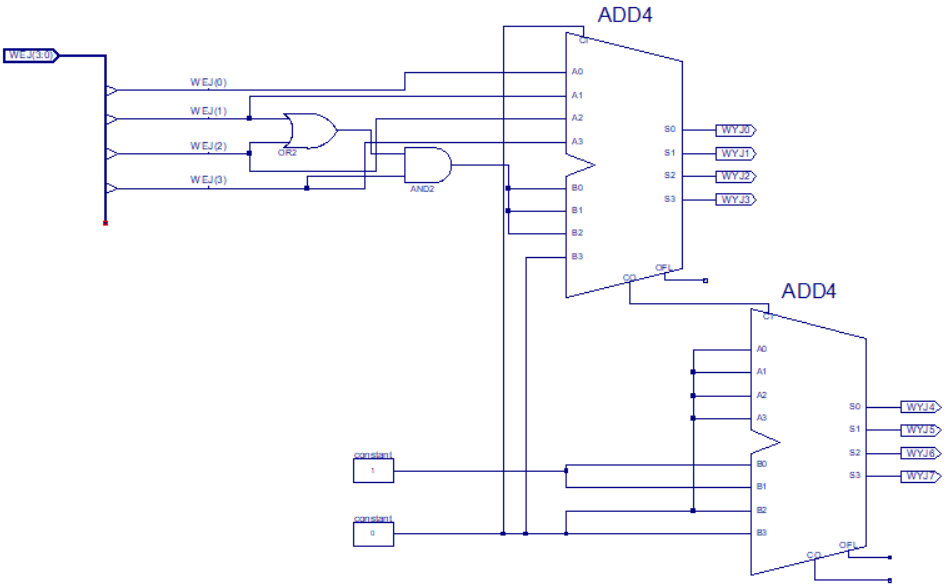
\includegraphics{zadanie3/zad3_scheme_diodes.png}
	}
\end{figure}
\subsubsection{Kod VHDL}
\lstinputlisting{zadanie3/testbench.vhd}
\subsubsection{Symulacja}
\begin{figure}[H]
	\centering
	\resizebox*{\textwidth}{!}{
		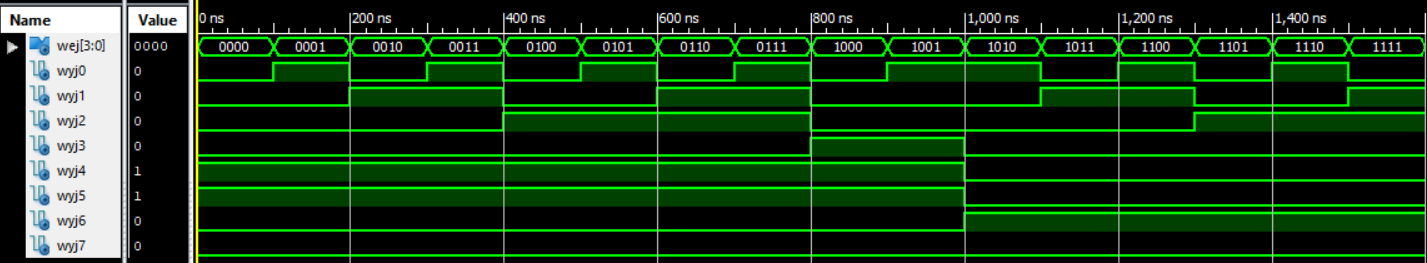
\includegraphics{zadanie3/zad3_simulation.png}
	}
\end{figure}
\subsection{Fizyczna implementacja}
\subsubsection{Kod UCF}
\lstinputlisting{zadanie3/zad3_diodes.ucf}
\subsection{Implementacja wyświetlacz}
Aby wykorzystać wyświetlacz do zaprezentowania wynikowego kodu dziesiętnego ASCII, musieliśmy zaimportować moduł Display4x7S ze strony laboratorium.

Aby moduł został poprawnie zaimplementowany musieliśmy go umieścić na schemacie, wczytać nowe wejścia do pliku VHDL oraz przypisać te wejścia do odpowiednich elementów zestawu fizycznego.
Moduł też wymaga od nas podłączenia do zegara wysokiej częstotliwości aby poprawnie wyświetlał wartości na ekranie zestawu.
\subsubsection{Schemat układu}
\begin{figure}[H]
	\centering
	\resizebox*{\textwidth}{!}{
		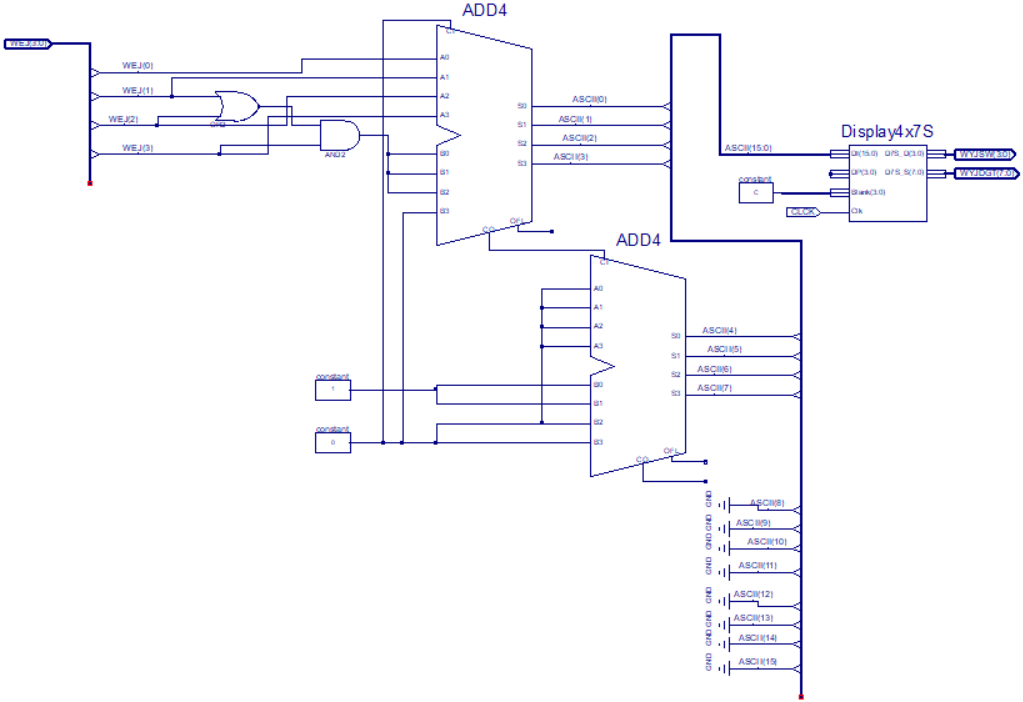
\includegraphics{zadanie3/zad3_scheme_display.png}
	}
\end{figure}
\subsubsection{Kod VHDL}
\lstinputlisting{zadanie3/testbench_display.vhd}
\subsubsection{Kod UCF}
\lstinputlisting{zadanie3/zad3_display.ucf}

Na początku mieliśmy zagwozdkę co mamy zrobić z bitami wejściowymi których jest 16 a my generujemy tylko 8. Uporaliśmy się z problemem poprzez wypełnienie pozostałych bitów zerami.

Efekt wyświetlenia wartości dziesiętnej kodu ASCII na ekranie zestawu był bardzo satysfakcjonujący.
\section{Zadanie 4}
\subsection{Polecenie}
Komparator dwóch 4-bitowych cyfr: 2 wejścia po 4 bity, 3 wyjścia 1-bitowe: 
mniejszy, większy, równy pracujący w kodzie Aikena.
\subsection{Rozwiązanie}
Na początku zadania zauważyliśmy że porównywanie wartości w kodzie Aikena wygląda identycznie jak w kodzie NKB.
Dzięki czemu udało nam się skonstruować nieskomplikowany schemat wraz z 3 wyjściami.
Do wykonania zadania wykorzystaliśmy wbudowany komparator w środowisku.
% \subsubsection{Schemat stanów}
% \subsubsection{Tabela prawdy}
% \subsubsection{Siatki Karnaugh}
\subsubsection{Schemat układu}
\begin{figure}[H]
   \centering
   \resizebox*{\textwidth}{!}{
	  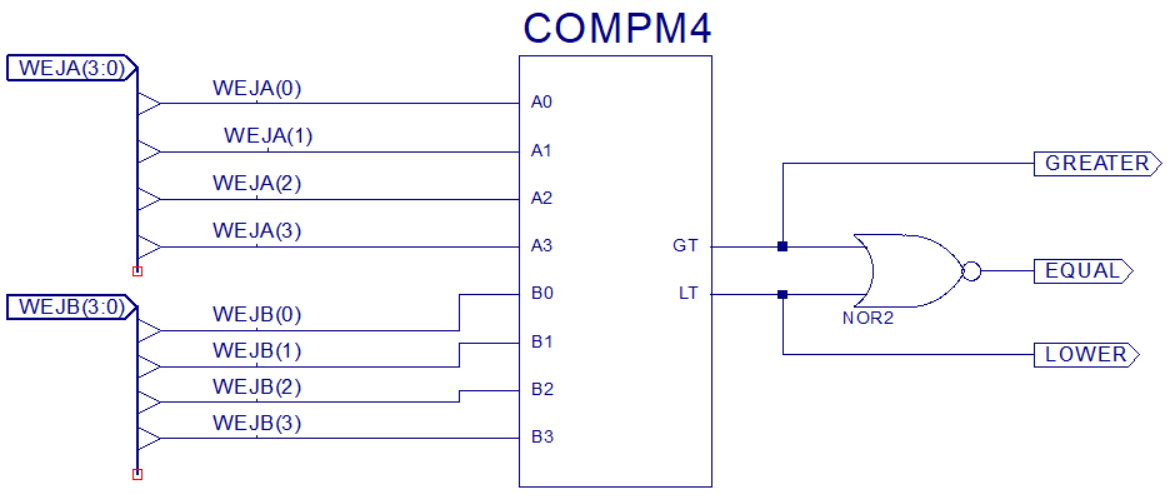
\includegraphics{zadanie4/zad4_scheme.png}
   }
\end{figure}
\subsubsection{Kod VHDL}
\lstinputlisting{zadanie4/testbench.vhd}
\subsubsection{Symulacja}
\begin{figure}[H]
   \centering
   \resizebox*{\textwidth}{!}{
	  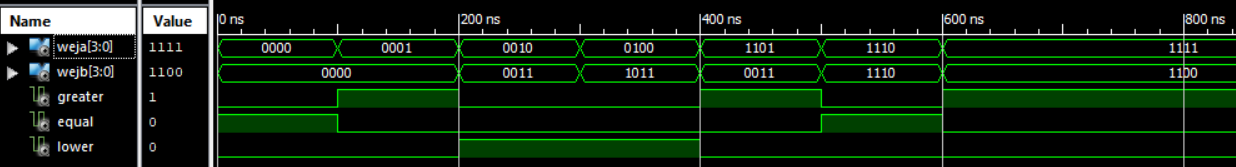
\includegraphics{zadanie4/zad4_simulation.png}
   }
\end{figure}
\subsection{Fizyczna implementacja}
\subsubsection{Kod UCF}
\lstinputlisting{zadanie4/ZL-9572.ucf}

Panel przycisków podzieliliśmy na 2 części tak samo jak w zadaniu nr. 2 aby móc bezproblemowo wprowadzać wartości.
Gdy wartość w lewej sekcji była mniejsza niż prawa, zapalała się prawa dioda sygnalizująca, że wartość po prawej stronie jest większa i vice versa, gdy wartości były równe to świeciła się dioda środkowa informująca o równości wartości.
\section{Wnioski}
Przy wykonywaniu zadań niezbędne okazały się inteligentne i proste rozwiązania problemów jak zauważenie w zadaniu 4, że porównywanie w kodzie Aikena jest identyczne z kodem KNB.

Małą trudność sprawiły nam moduły implementujące działanie wyświetlacza LCD oraz wprowadzanie wejścia za pomocą klawiatury przez terminal, lecz po przeczytaniu instrukcji i wykonaniu opisanych kroków dobrnęliśmy do rozwiązania problemu.

Najtrudniejszym zadaniem okazało się zadanie 2 gdyż wymagało to od nas dokonania kilku założeń ze względu na specyfikację kodu:
Ignorowanie wyjścia gdy będzie przepełnienie oraz odejmowanie/dodawanie wartości 6 gdy zakres przekroczy wartość 4.
\end{document}